\chapter{Analytics in use}~\label{chapter-analytics-in-use}
\julian{This chapter covers \uuse and \iuse}

\section{Sensemaking and decision-taking by developers}~\label{sensemaking-and-decision-taking-by-developers-section}
Beacon-finding and drill-down parallel similar practices used by app developers when they use mobile analytics as inputs to their development work and as feedback for [their] previous development work.

\begin{figure}
    \centering
    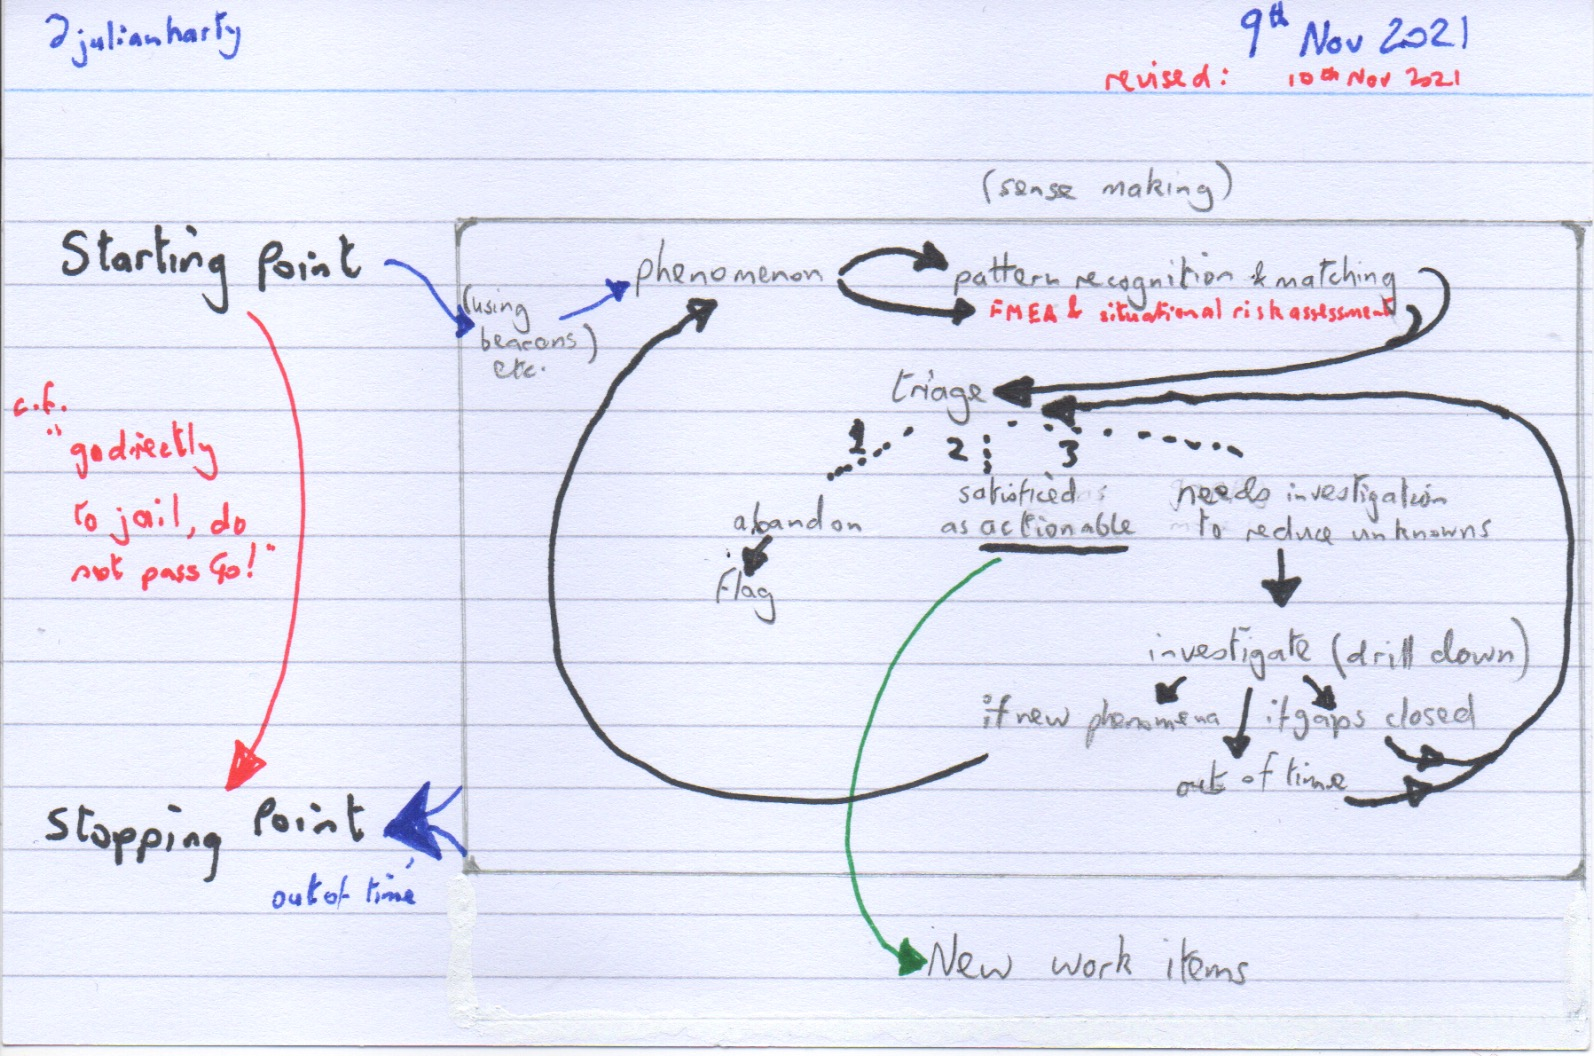
\includegraphics[width=15cm]{images/rough-sketches/practical-sense-making-process-10-nov-2021.jpeg}
    \caption{Sense-making process when development teams apply mobile analytics}
    \label{fig:practical-sense-making-process-when-dev-teams-apply-mobile-analytics}
\end{figure}


Figure~\ref{fig:practical-sense-making-process-when-dev-teams-apply-mobile-analytics} illustrates the sense-making and triage process used by development teams which shares various similarities with sense-making from a research perspective. These similarities mean the researcher and the practitioner may also share similar practices in terms of their analysis of phenomena found in mobile analytics tools. The triage and drill-down may be repeated several times where there is sufficient potential value in performing further investigation. 

The impact of reported failures is combined with situational-risk-assessment as a part of the decision-making process performed by developers during triage; for instance to consider whether this reported issue is worth addressing in the current development cycle, (\textit{e.g.} in the current sprint for teams who use sprints for work planning. Developers have to consider multiple criteria including personal, project, and product implications of making code and/or operational changes. An untested hypothesis for their approach is introduced in the discussion chapter on page \pageref{discussion-decision-making-by-dev-teams-section}.

\newthought{Premature satisfaction}

The following example needs moving to a later chapter once I've sketched out the research equivalent of Figure~\ref{fig:practical-sense-making-process-when-dev-teams-apply-mobile-analytics}.
Many of the developers were often satisficed with what the mobile analytics tools reported - where they accepted local optima (determined through a combination of observation and asking the app devs), \textit{e.g.} they accepted the `top' crash cluster as the worst one. Therefore, if there are flaws in what is being reported the effects of those flaws may permeate into the results of what the developers \textit{do} and \textit{don't} do. 